\documentclass[aspectratio=169,11pt]{beamer}
% Shared style for the Introduction to Information Geometry lecture slides.
% Compile the lecture .tex files from this directory.
\providecommand{\courseweek}{1}
\usepackage[T1]{fontenc}
\usepackage[utf8]{inputenc}
\usepackage[sc]{mathpazo}
\renewcommand{\sfdefault}{lmss}
\renewcommand{\ttdefault}{lmtt}
\usepackage{amsmath,amssymb,mathtools}
\usepackage{tikz}
\usetikzlibrary{arrows.meta,calc,positioning}
\usepackage{pgfplots}
\pgfplotsset{compat=1.18}
\usepackage{booktabs}

\definecolor{courseink}{HTML}{173749}
\definecolor{coursemuted}{HTML}{526674}
\definecolor{courseteal}{HTML}{0E7287}
\definecolor{coursecopper}{HTML}{B66B43}
\definecolor{courseline}{HTML}{D4E0E3}
\definecolor{coursepale}{HTML}{EFF5F5}

\setbeamercolor{normal text}{fg=courseink,bg=white}
\setbeamercolor{structure}{fg=courseteal}
\setbeamercolor{frametitle}{fg=courseink,bg=white}
\setbeamercolor{title}{fg=courseink}
\setbeamercolor{subtitle}{fg=coursemuted}
\setbeamercolor{block title}{fg=courseink,bg=white}
\setbeamercolor{block body}{fg=courseink,bg=white}
\setbeamercolor{alerted text}{fg=coursecopper}
\setbeamerfont{title}{family=\rmfamily,series=\bfseries,size=\fontsize{32}{37}}
\setbeamerfont{frametitle}{family=\rmfamily,series=\bfseries,size=\fontsize{26}{31}}
\setbeamerfont{normal text}{size=\fontsize{18}{22}}
\setbeamerfont{subtitle}{size=\fontsize{17}{21}}
\setbeamersize{text margin left=0.78cm,text margin right=0.78cm}
\setbeamertemplate{navigation symbols}{}
\setbeamertemplate{itemize items}[circle]
\setbeamertemplate{enumerate items}[default]
\setbeamertemplate{blocks}[default]
\setlength{\parskip}{0.22em}
\setbeamertemplate{footline}{%
  \leavevmode\hbox to \paperwidth{\hspace{.78cm}%
  {\color{coursemuted}\fontsize{8.5}{10}\selectfont Introduction to Information Geometry \hspace{.32cm} / \hspace{.32cm} Week \courseweek}%
  \hfill{\color{coursemuted}\fontsize{8.5}{10}\selectfont \insertframenumber\hspace{.17cm}/\hspace{.17cm}\inserttotalframenumber}\hspace{.78cm}}%
  \vskip.17cm
}
\setbeamertemplate{frametitle}{%
  \vspace{.13cm}
  \insertframetitle\par
  \vspace{.08cm}
}
\setbeamertemplate{title page}{%
  \vspace*{1.00cm}
  {\color{courseteal}\fontsize{10}{13}\selectfont\bfseries
  INTRODUCTION TO INFORMATION GEOMETRY\par}
  \vspace{.40cm}
  {\usebeamerfont{title}\usebeamercolor[fg]{title}\inserttitle\par}
  \vspace{.22cm}
  {\usebeamerfont{subtitle}\usebeamercolor[fg]{subtitle}\insertsubtitle\par}
  \vfill
  {\color{coursemuted}\fontsize{13}{16}\selectfont Christopher Lee\par}
  \vspace{.34cm}
}

\pgfplotsset{
  courseplot/.style={
    width=11.05cm,
    height=5.15cm,
    axis line style={coursemuted!75},
    tick style={coursemuted!65},
    ticklabel style={font=\scriptsize,color=coursemuted},
    label style={font=\normalsize,color=courseink},
    grid=major,
    major grid style={courseline!70,line width=.4pt},
    line width=1.45pt,
    legend style={font=\small,draw=none,fill=none,at={(.98,.03)},anchor=south east},
    clip=true
  }
}

\newcommand{\highlightmath}[1]{{\color{courseteal}#1}}
\newcommand{\thinrule}{\par\vspace{.25cm}{\color{courseline}\rule{\linewidth}{.8pt}}\par}

% A one-dimensional state space.  x=0 and x=1 are placed at 0 and 9 units.
\newcommand{\stateinterval}[1]{%
 \begin{tikzpicture}[x=1cm,y=1cm]
   \draw[courseink,line width=1.25pt] (0,0)--(9,0);
   \foreach \pos/\lab in {0/0,9/1} {
     \fill[courseink] (\pos,0) circle(2.7pt);
     \node[below=9pt,text=coursemuted] at (\pos,0) {\(\lab\)};
   }
   #1
 \end{tikzpicture}%
}

% Paired pages are separate frames in the PDF, with matching titles.
% Supply the whole frame body for each version; the instructor may edit them
% independently without changing overlay logic.
\newcommand{\coursepair}[3]{%
  \begin{frame}{#1}#2\end{frame}%
  \begin{frame}{#1}#3\end{frame}%
}

% Equilateral representation of the categorical simplex, in barycentric
% coordinates with vertices A=(0,0), B=(1,0), C=(1/2,sqrt(3)/2).
\newcommand{\coursesimplex}[1]{%
 \begin{tikzpicture}[scale=4.9]
  \fill[coursepale] (0,0)--(1,0)--(.5,.8660254)--cycle;
  \draw[courseink,line width=.65pt] (0,0)--(1,0)--(.5,.8660254)--cycle;
  \node[below left,font=\small] at (0,0) {A};
  \node[below right,font=\small] at (1,0) {B};
  \node[above,font=\small] at (.5,.8660254) {C};
  #1
 \end{tikzpicture}%
}

\title{Frequency-Dependent Fitness\\and Stability}
\subtitle{Week 1 \(\cdot\) Lecture 2}
\date{}

\begin{document}

% 1
\begin{frame}[plain]
\titlepage
\end{frame}

% 2
\begin{frame}{The scalar replicator model}
From the first lecture,
\vspace{.45cm}
\begin{center}
{\fontsize{29}{36}\selectfont
\(\displaystyle \highlightmath{x'=x(1-x)\Delta(x)}\)}
\end{center}
\vspace{.43cm}
\[
\Delta(x)=f_A(x)-f_B(x).
\]
\vspace{.35cm}
The fitness difference may vary with the current proportion.
This makes the direction of motion depend on the state.
\end{frame}

% 3
\begin{frame}{Fitnesses that depend on frequency}
Consider
\[
\highlightmath{f_A(x)=3-2x},
\qquad
\highlightmath{f_B(x)=2x}.
\]
\vspace{-.30cm}
\begin{center}
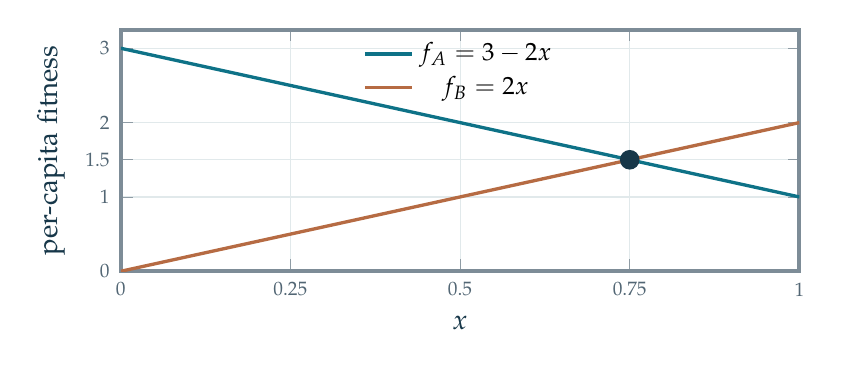
\begin{tikzpicture}
\begin{axis}[courseplot,width=10.2cm,height=4.65cm,
 xmin=0,xmax=1,ymin=0,ymax=3.25,
 xlabel={$x$},ylabel={per-capita fitness},
 xtick={0,.25,.5,.75,1},ytick={0,1,1.5,2,3},
 legend style={at={(.5,1)},anchor=north}]
\addplot[courseteal,very thick,domain=0:1] {3-2*x};
\addlegendentry{\(f_A=3-2x\)}
\addplot[coursecopper,very thick,domain=0:1] {2*x};
\addlegendentry{\(f_B=2x\)}
\addplot[only marks,mark=*,mark size=2.8pt,courseink]
 coordinates {(.75,1.5)};
\end{axis}
\end{tikzpicture}
\end{center}
\end{frame}

% 4
\begin{frame}{The fitness difference}
\[
\highlightmath{\Delta(x)=(3-2x)-2x=3-4x}.
\]
\vspace{.35cm}
\begin{center}
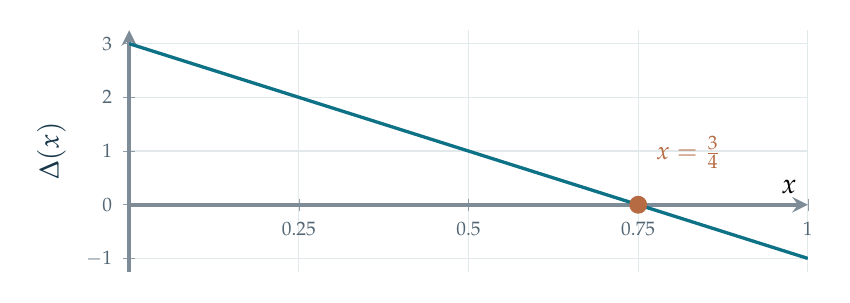
\begin{tikzpicture}
\begin{axis}[courseplot,width=10.2cm,height=4.65cm,
 xmin=0,xmax=1,ymin=-1.25,ymax=3.25,
 xlabel={$x$},ylabel={\(\Delta(x)\)},xtick={0,.25,.5,.75,1},
 ytick={-1,0,1,2,3},axis x line=middle,axis y line=left]
\addplot[courseteal,very thick,domain=0:1] {3-4*x};
\addplot[only marks,mark=*,mark size=2.5pt,coursecopper] coordinates {(.75,0)};
\node[anchor=south west,text=coursecopper,font=\small] at (axis cs:.76,.47) {\(x=\tfrac34\)};
\end{axis}
\end{tikzpicture}
\end{center}
\end{frame}

% 5
\begin{frame}{Equilibria of the frequency model}
The equation becomes
\vspace{.45cm}
\[
\highlightmath{x'=F(x)=x(1-x)(3-4x)}.
\]
\vspace{.40cm}
An equilibrium \(e\) satisfies \(F(e)=0\).

\vspace{.42cm}
\[
e=\;?
\]
\end{frame}

% Reveal: frequency-dependent equilibria
\begin{frame}{Equilibria of the frequency model}
The equation becomes
\vspace{.45cm}
\[
\highlightmath{x'=F(x)=x(1-x)(3-4x)}.
\]
\vspace{.40cm}
An equilibrium \(e\) satisfies \(F(e)=0\).

\vspace{.42cm}
\[
\highlightmath{e=0,\quad\frac34,\quad1.}
\]
\end{frame}

% 6
\begin{frame}{The phase line}
The equilibria are \(0\), \(\frac34\), and \(1\).
\vspace{.57cm}
\begin{center}
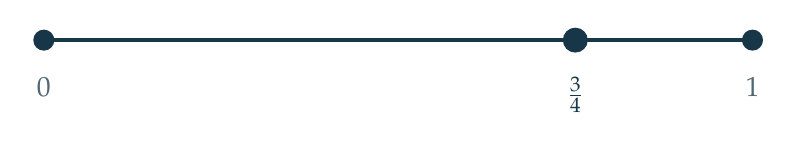
\begin{tikzpicture}[x=1cm,y=1cm]
 \draw[courseink,line width=1.35pt] (0,0)--(9,0);
 \fill[courseink] (0,0) circle(3.8pt);
 \fill[courseink] (6.75,0) circle(4.5pt);
 \fill[courseink] (9,0) circle(3.8pt);
 \node[below=10pt,text=coursemuted] at (0,0) {\(0\)};
 \node[below=10pt,text=courseink] at (6.75,0) {\(\frac34\)};
 \node[below=10pt,text=coursemuted] at (9,0) {\(1\)};
\end{tikzpicture}
\end{center}
\vspace{.8cm}
\begin{center}
Draw the arrows using the sign of \(F(x)\). Which equilibrium attracts?
\end{center}
\end{frame}

% Reveal: frequency-dependent phase line
\begin{frame}{The phase line}
The equilibria are \(0\), \(\frac34\), and \(1\).
\vspace{.57cm}
\begin{center}
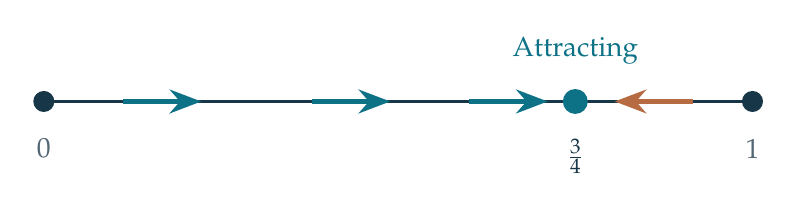
\begin{tikzpicture}[x=1cm,y=1cm]
 \draw[courseink,line width=1.35pt] (0,0)--(9,0);
 \fill[courseink] (0,0) circle(3.8pt);
 \fill[courseteal] (6.75,0) circle(4.5pt);
 \fill[courseink] (9,0) circle(3.8pt);
 \foreach \x in {1.5,3.9,5.9}
  \draw[-{Stealth[length=4mm]},courseteal,line width=2pt] (\x-.50,0)--(\x+.50,0);
 \draw[-{Stealth[length=4mm]},coursecopper,line width=2pt] (8.25,0)--(7.25,0);
 \node[below=10pt,text=coursemuted] at (0,0) {\(0\)};
 \node[below=10pt,text=courseink] at (6.75,0) {\(\frac34\)};
 \node[below=10pt,text=coursemuted] at (9,0) {\(1\)};
 \node[above=10pt,text=courseteal] at (6.75,0) {Attracting};
\end{tikzpicture}
\end{center}
\vspace{.8cm}
\begin{center}
\(F(x)>0\) for \(0<x<\frac34\),
\qquad
\(F(x)<0\) for \(\frac34<x<1\).
\end{center}
\end{frame}

% 7
\begin{frame}{Velocity as a function of state}
\vspace{-.24cm}
\begin{center}
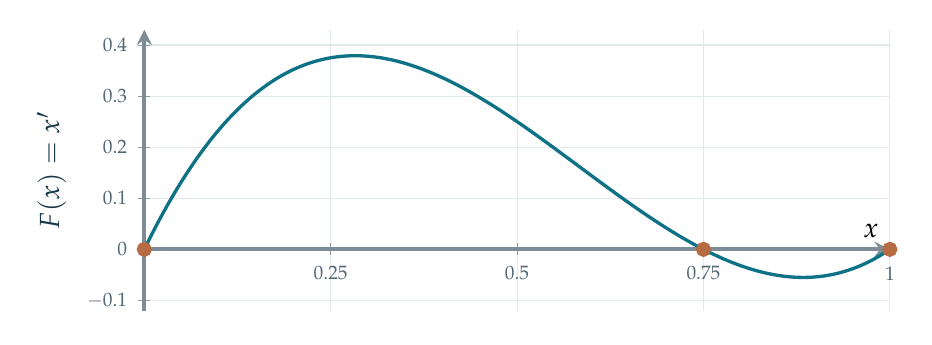
\begin{tikzpicture}
\begin{axis}[courseplot,xmin=0,xmax=1,ymin=-.12,ymax=.43,
 xlabel={$x$},ylabel={$F(x)=x'$},xtick={0,.25,.5,.75,1},
 ytick={-.1,0,.1,.2,.3,.4},axis x line=middle,axis y line=left]
\addplot[courseteal,very thick,domain=0:1,samples=160] {x*(1-x)*(3-4*x)};
\addplot[only marks,mark=*,mark size=2pt,coursecopper]
 coordinates {(0,0)(.75,0)(1,0)};
\end{axis}
\end{tikzpicture}
\end{center}
\vspace{-.18cm}
The height of the graph gives the slope of a solution at that state.
\end{frame}

% 8
\begin{frame}{Reading instantaneous velocities}
For
\[
F(x)=x(1-x)(3-4x),
\]
calculate
\vspace{.2cm}
\[
F(0.4)=\;?\qquad\text{and}\qquad F(0.9)=\;?.
\]
\vspace{.42cm}
Which solution is increasing? Which is decreasing?
\end{frame}

% Reveal: numerical velocities
\begin{frame}{Reading instantaneous velocities}
For
\[
F(x)=x(1-x)(3-4x),
\]
calculate
\vspace{.2cm}
\[
F(0.4)=\highlightmath{0.336}\qquad\text{and}\qquad
F(0.9)=\highlightmath{-0.054}.
\]
\vspace{.42cm}
The solution at \(x=0.4\) increases; the one at \(x=0.9\) decreases.
\end{frame}

% 9
\begin{frame}{Trajectories from three starting states}
\vspace{-.28cm}
\begin{center}
\begin{tikzpicture}
\begin{axis}[courseplot,xmin=0,xmax=10,ymin=0,ymax=1.04,
 xlabel={time \(t\)},ylabel={$x(t)$},
 xtick={0,2,4,6,8,10},ytick={0,.25,.5,.75,1},
 legend style={at={(.98,.24)},anchor=south east}]
\addplot[courseteal,very thick] table[x=t,y=x01,col sep=comma] {coexistence_trajectories.csv};
\addlegendentry{\(x(0)=0.1\)}
\addplot[courseink,very thick] table[x=t,y=x04,col sep=comma] {coexistence_trajectories.csv};
\addlegendentry{\(x(0)=0.4\)}
\addplot[coursecopper,very thick] table[x=t,y=x09,col sep=comma] {coexistence_trajectories.csv};
\addlegendentry{\(x(0)=0.9\)}
\addplot[coursemuted,dashed,domain=0:10] {.75};
\end{axis}
\end{tikzpicture}
\end{center}
\vspace{-.17cm}
Every interior trajectory approaches the equilibrium composition \(x=\frac34\).
\end{frame}

% 10
\begin{frame}{Three descriptions of the same motion}
\vspace{.1cm}
\begin{enumerate}
\setlength{\itemsep}{.56cm}
\item The \textcolor{courseteal}{phase line} records the direction of motion at each state.
\item The graph of \(\textcolor{courseteal}{F(x)}\) gives the instantaneous velocity at that state.
\item The solution \(\textcolor{courseteal}{x(t)}\) traces one trajectory through time.
\end{enumerate}
\vspace{.50cm}
When \(x(t)=0.4\), the time-graph slope must equal
\[
x'(t)=F(0.4)=0.336.
\]
\end{frame}

% 11
\begin{frame}{Stability on the interval}
An equilibrium \(e\) is \emph{stable} if solutions starting sufficiently
close remain close for all future time.
\vspace{.45cm}
\par
It is \emph{asymptotically stable} if those nearby solutions also
converge to \(e\).
\vspace{.52cm}
For the coexistence model, the phase-line arrows point toward
\[
\highlightmath{e=\frac34}.
\]
\end{frame}

% 12
\begin{frame}{Linearization near an equilibrium}
Let \(x=e+u\), where \(u\) is a small displacement.
\vspace{.35cm}
Taylor expansion gives
\[
F(e+u)=F(e)+F'(e)u+O(u^2).
\]
\vspace{.37cm}
Because \(F(e)=0\), the leading-order equation is
\vspace{.18cm}
\[
\highlightmath{u'=F'(e)u}.
\]
\vspace{.32cm}
\begin{center}
\(F'(e)<0\) predicts decay, while \(F'(e)>0\) predicts growth.
\end{center}
\end{frame}

% 13
\begin{frame}{The derivative at coexistence}
\[
F(x)=x(1-x)(3-4x), \qquad e=\frac34.
\]
\vspace{.37cm}
Find
\[
F'(e)=\;?
\]
\vspace{.33cm}
You may differentiate the expanded polynomial or use the product rule
at the equilibrium.
\end{frame}

% Reveal: derivative at coexistence
\begin{frame}{The derivative at coexistence}
\[
F(x)=x(1-x)(3-4x), \qquad e=\frac34.
\]
\vspace{.37cm}
Find
\[
\highlightmath{F'(e)=\frac34\left(1-\frac34\right)(-4)=-\frac34.}
\]
\vspace{.33cm}
The negative derivative predicts exponential decay of small displacements.
\end{frame}

% 14
\begin{frame}{Exponential approach to equilibrium}
At \(e=\frac34\), differentiation gives
\[
F'(e)=-\frac34.
\]
\vspace{.38cm}
For a small displacement \(u=x-\frac34\),
\[
\highlightmath{u(t)\approx u(0)e^{-3t/4}}.
\]
\vspace{.52cm}
The displacement decreases by a factor of \(e\) in approximately
\[
\highlightmath{\frac43\text{ time units}.}
\]
\end{frame}

% 15
\begin{frame}{The local decay curve}
\vspace{-.10cm}
\begin{center}
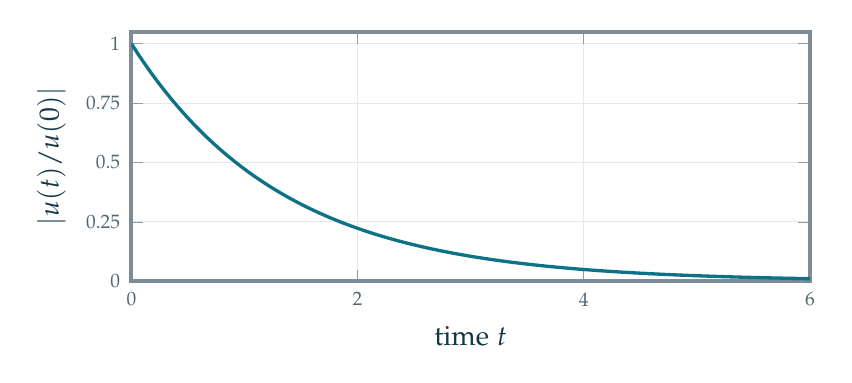
\begin{tikzpicture}
\begin{axis}[courseplot,width=10.2cm,height=4.75cm,
 xmin=0,xmax=6,ymin=0,ymax=1.05,
 xlabel={time \(t\)},ylabel={\(\lvert u(t)/u(0)\rvert\)},
 xtick={0,2,4,6},ytick={0,.25,.5,.75,1}]
\addplot[courseteal,very thick,domain=0:6,samples=100] {exp(-.75*x)};
\end{axis}
\end{tikzpicture}
\end{center}
\vspace{-.18cm}
This approximation describes motion close to the equilibrium.
\end{frame}

% 16
\begin{frame}{Why solutions remain in \([0,1]\)}
\vspace{.25cm}
\[
F(x)=x(1-x)\Delta(x),
\quad
\highlightmath{F(0)=F(1)=0}.
\]
\vspace{.50cm}
Thus \(x(t)\equiv0\) and \(x(t)\equiv1\) are constant solutions.
\vspace{.48cm}
For a smooth fitness difference, uniqueness of solutions prevents
an interior trajectory from crossing either endpoint.
\vspace{.42cm}
The probability interval \(\highlightmath{[0,1]}\) is forward invariant.
\end{frame}

% 17
\begin{frame}{A model with an unstable threshold}
Compare the coexistence equation with
\vspace{.07cm}
\[
\highlightmath{x'=x(1-x)(4x-2)}.
\]
\vspace{.07cm}
Its interior equilibrium is \(e=\frac12\).
\vspace{.04cm}
\begin{center}
\stateinterval{
 \fill[coursecopper] (4.5,0) circle(4.5pt);
 \node[above=11pt,text=coursecopper] at (4.5,0) {\(x=\frac12\)};
}
\end{center}
\vspace{.06cm}
Draw the direction arrows and classify all three equilibria.
\end{frame}

% Reveal: unstable threshold
\begin{frame}{A model with an unstable threshold}
Compare the coexistence equation with
\vspace{.07cm}
\[
\highlightmath{x'=x(1-x)(4x-2)}.
\]
\vspace{.07cm}
Its interior equilibrium is \(e=\frac12\).
\vspace{.04cm}
\begin{center}
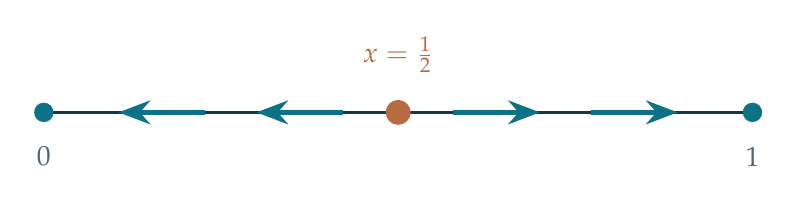
\begin{tikzpicture}[x=1cm,y=1cm]
 \draw[courseink,line width=1.25pt] (0,0)--(9,0);
 \fill[courseteal] (0,0) circle(3.5pt);
 \fill[coursecopper] (4.5,0) circle(4.5pt);
 \fill[courseteal] (9,0) circle(3.5pt);
 \node[below=9pt,text=coursemuted] at (0,0) {\(0\)};
 \node[below=9pt,text=coursemuted] at (9,0) {\(1\)};
 \node[above=11pt,text=coursecopper] at (4.5,0) {\(x=\frac12\)};
 \foreach \x in {1.5,3.25}
  \draw[-{Stealth[length=4mm]},courseteal,line width=2pt] (\x+.55,0)--(\x-.55,0);
 \foreach \x in {5.75,7.5}
  \draw[-{Stealth[length=4mm]},courseteal,line width=2pt] (\x-.55,0)--(\x+.55,0);
\end{tikzpicture}
\end{center}
\vspace{.06cm}
The endpoints attract; \(x=\frac12\) is unstable.
\end{frame}

% 18
\begin{frame}{A proportion is a probability distribution}
Selecting one individual at random gives
\vspace{.45cm}
\begin{center}
{\fontsize{27}{34}\selectfont
\(\displaystyle \highlightmath{P=(x,1-x)}\)}
\end{center}
\vspace{.28cm}
\begin{center}
\stateinterval{
 \fill[courseteal] (2.25,0) circle(4pt);
 \fill[coursecopper] (6.75,0) circle(4pt);
 \node[above=10pt,text=courseteal] at (2.25,0) {\((.25,.75)\)};
 \node[above=10pt,text=coursecopper] at (6.75,0) {\((.75,.25)\)};
}
\end{center}
\vspace{.15cm}
A replicator trajectory is therefore a curve of two-outcome distributions.
\end{frame}

% 19
\begin{frame}{Week 1: three mathematical tools}
\vspace{.15cm}
\begin{enumerate}
\setlength{\itemsep}{.62cm}
\item A \emph{replicator equation} determines how the proportion changes:
\[
x'=x(1-x)(f_A-f_B).
\]
\item A \emph{phase line} identifies equilibria and directions of motion.
\item A \emph{linearization} estimates the local rate of approach or departure:
\[
u'\approx F'(e)u.
\]
\end{enumerate}
\vspace{.12cm}
Week 2 will obtain the fitness functions from payoff matrices.
\end{frame}

\end{document}
